\documentclass[a4paper,11pt,twoside]{article}
%\documentclass[a4paper,11pt,twoside,se]{article}

\usepackage{UmUStudentReport}
\usepackage{verbatim}   % Multi-line comments using \begin{comment}
\usepackage{courier}    % Nicer fonts are used. (not necessary)
\usepackage{pslatex}    % Also nicer fonts. (not necessary)
\usepackage[pdftex]{graphicx}   % allows including pdf figures
\usepackage{listings}
\usepackage{pgf-umlcd}
\usepackage{blindtext}
\usepackage{enumitem}
%\usepackage{lmodern}   % Optional fonts. (not necessary)
%\usepackage{tabularx}
%\usepackage{microtype} % Provides some typographic improvements over default settings
%\usepackage{placeins}  % For aligning images with \FloatBarrier
%\usepackage{booktabs}  % For nice-looking tables
%\usepackage{titlesec}  % More granular control of sections.

% DOCUMENT INFO
% =============
\department{Department of Computing Science}
\coursename{Development of Mobile Appliations 7.5 p}
\coursecode{5DV155}
\title{User Interface for Mobile Systems}
\author{Lorenz Gerber ({\tt{dv15lgr@cs.umu.se}} {\tt{lozger03@student.umu.se}})}
\date{2017-07-20}
%\revisiondate{2016-01-18}
\instructor{Johan Eliasson / Jonathan Westin}


% DOCUMENT SETTINGS
% =================
\bibliographystyle{plain}
%\bibliographystyle{ieee}
\pagestyle{fancy}
\raggedbottom
\setcounter{secnumdepth}{2}
\setcounter{tocdepth}{2}
%\graphicspath{{images/}}   %Path for images

\usepackage{float}
\floatstyle{ruled}
\newfloat{listing}{thp}{lop}
\floatname{listing}{Listing}



% DEFINES
% =======
%\newcommand{\mycommand}{<latex code>}

% DOCUMENT
% ========
\begin{document}
\lstset{language=C}
\maketitle
\thispagestyle{empty}
\newpage
\tableofcontents
\thispagestyle{empty}
\newpage

\clearpage
\pagenumbering{arabic}

\section{Introduction}
The aim of this assignment is to translate a desktop mail client application to
a mobile app. This includes both functional and design related aspects. The
functionality shalls be described in terms of android elements and concepts such
as activities, layouts, menues, dialogs, fragments and messages. A main aspect is
to decide and reason which functionality should be stripped from the desktop version
and eventual additional functionality needed in the mobile app.

The design shall account for usability aspects following concepts from the
course litterature \cite{clark2015} and platform guidelines \cite{materialdesign}.
The report has to include several prototype designs of which at least one shall be
made in `Android Studio' and one by hand or any design/drawing application of choice.

Further, one section of the report shall describe differences and changes in the
design when the proposed Android application would be ported to another mobile
platform of choice.

\section{The Desktop Mail Client - Apple Mail}
Here the 'Apple Mail' client was chosen as the application to be ported into
an Android mobile app. The version at hand was 10.3 (3273) in a macOS Sierra
Environment (10.12.5). Initially, a systematic inventory of the available
functionality in Apple Mail was conducted.

\subsection{Description of main UI of Apple Mail}
The main UI of Apple Mail can be seen in figure \ref{fig_apple_mail_scren}.
It consists of three columns, of which only the `Mail List' and `Mail Details'
column are shown by default. The `Mail List' shows all mails of the active mailbox.
the list entry can be customised in the `Preferences', accessible through the `File'
drop down menu. The `Mail List' has by default a sort/filter bar with a drop down
menu for various list sort methods and an icon button to apply filters. The `Mail
List' scrolls vertically when not all mails of the mailbox fit on the screen.
Inspired by the Apple iOS interface, mail list items implement horizontal swipe
actions. By default, to the right for deleting and to the left for toggling
read/unread.

The `Mail Details' frame shows the detail view of one email, the one selected in
the `Mail List'. This view scrolls if needed both vertically and horizontally.
Various options regarding the visualization can be chosen in the `Preferences'
menu. By default, the header of the mail contains a number of `hyperlink' style
functionality for toggling visibility of some less often needed information but
also as shortcut for the common mail actions `delete', `reply', `reply to all' and
`forward'.

The `Mailbox List' column can be toggled visible/invisible
by a button in the `Favorites' bar which otherwise contains text buttons for the
available mailboxes.


\begin{figure}
  \label{fig:apple_main_screen}
  \centering
    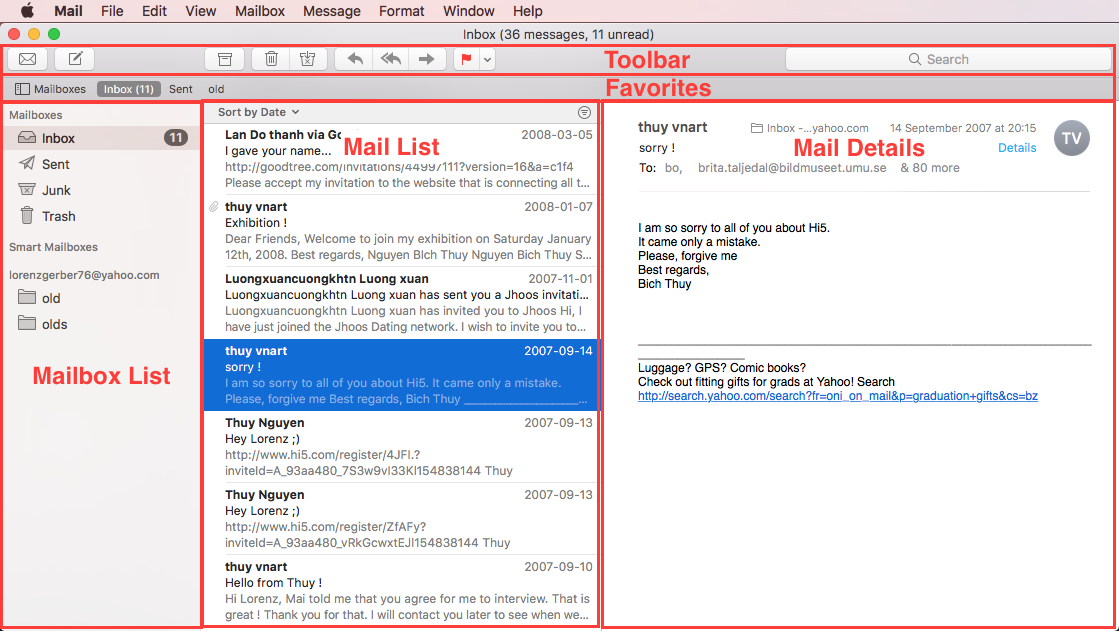
\includegraphics[width=1\textwidth]{main_screen}
    \caption{\textit{The main view of Apple Mail has three columns: `Mailbox List',
    `Mail List' and `Mail Details'. The `Mailbox List' column is however
    hidden in the standard configuration.}}
\end{figure}

\subsection{Description of Menu accessible Functionality in Apple Mail}

\section{Design with Android Elements}
How to splitup the functionality into activities, layouts, menues, dialogs, fragments and messages.
Elaborate which functions that are most important and that should be included.
Which functions can be left out to compensate for the mobile context
Is there needed some additional functionality for the mobile context
reflect on the different aspects regarding usability
describe how the interaction shall happen.
Motivate design descisions.

\section{Some design examples from Android Studio UI Designer, some pen paper designs}

\section{describe how all main functionality in the app}


\section{Describe needed changes for another mobile platform}


\addcontentsline{toc}{section}{\refname}
\bibliography{references}

\end{document}
